\subsection{Motivations for Next Generation CSACs}
\label{subsec:motivations}

While current \acrshort{csac} technology offers significant advantages in terms of miniaturization with respect traditional atomic clocks, there is still room for improvement under every aspect of the clock (stability, accuracy, SWaP, etc.).

As it has been with the development of the first \acrshort{csac}, DARPA is again the main driver for the development of next-generation \acrshort{csacs}.
Among the funded projects and collaborations with multiple research institutions, three main programs are worth mentioning:

\begin{itemize}
    \item IMPACT: aimed to develop a \acrshort{csac} with a volume of $20cm^3$, a power consumption of $250mW$ and a long-term stability of $\sigma_y(\tau=1month) < 160ns$.
    \item ACES: aimed to develop a palm-sized, battery-powered \acrshort{csac} with a $1000x$ performance improvement with respect to the current commercial available \acrshort{csac}.
    \item ROCkN: continuation of the ACES program, with the aim of further improving the performances of the \acrshort{csac}.
\end{itemize}

The stability targets aimed by these DARPA programs are illustrated in Figure \ref{fig:DARPA-stability-target}.

\begin{figure}[H]
    \centering
    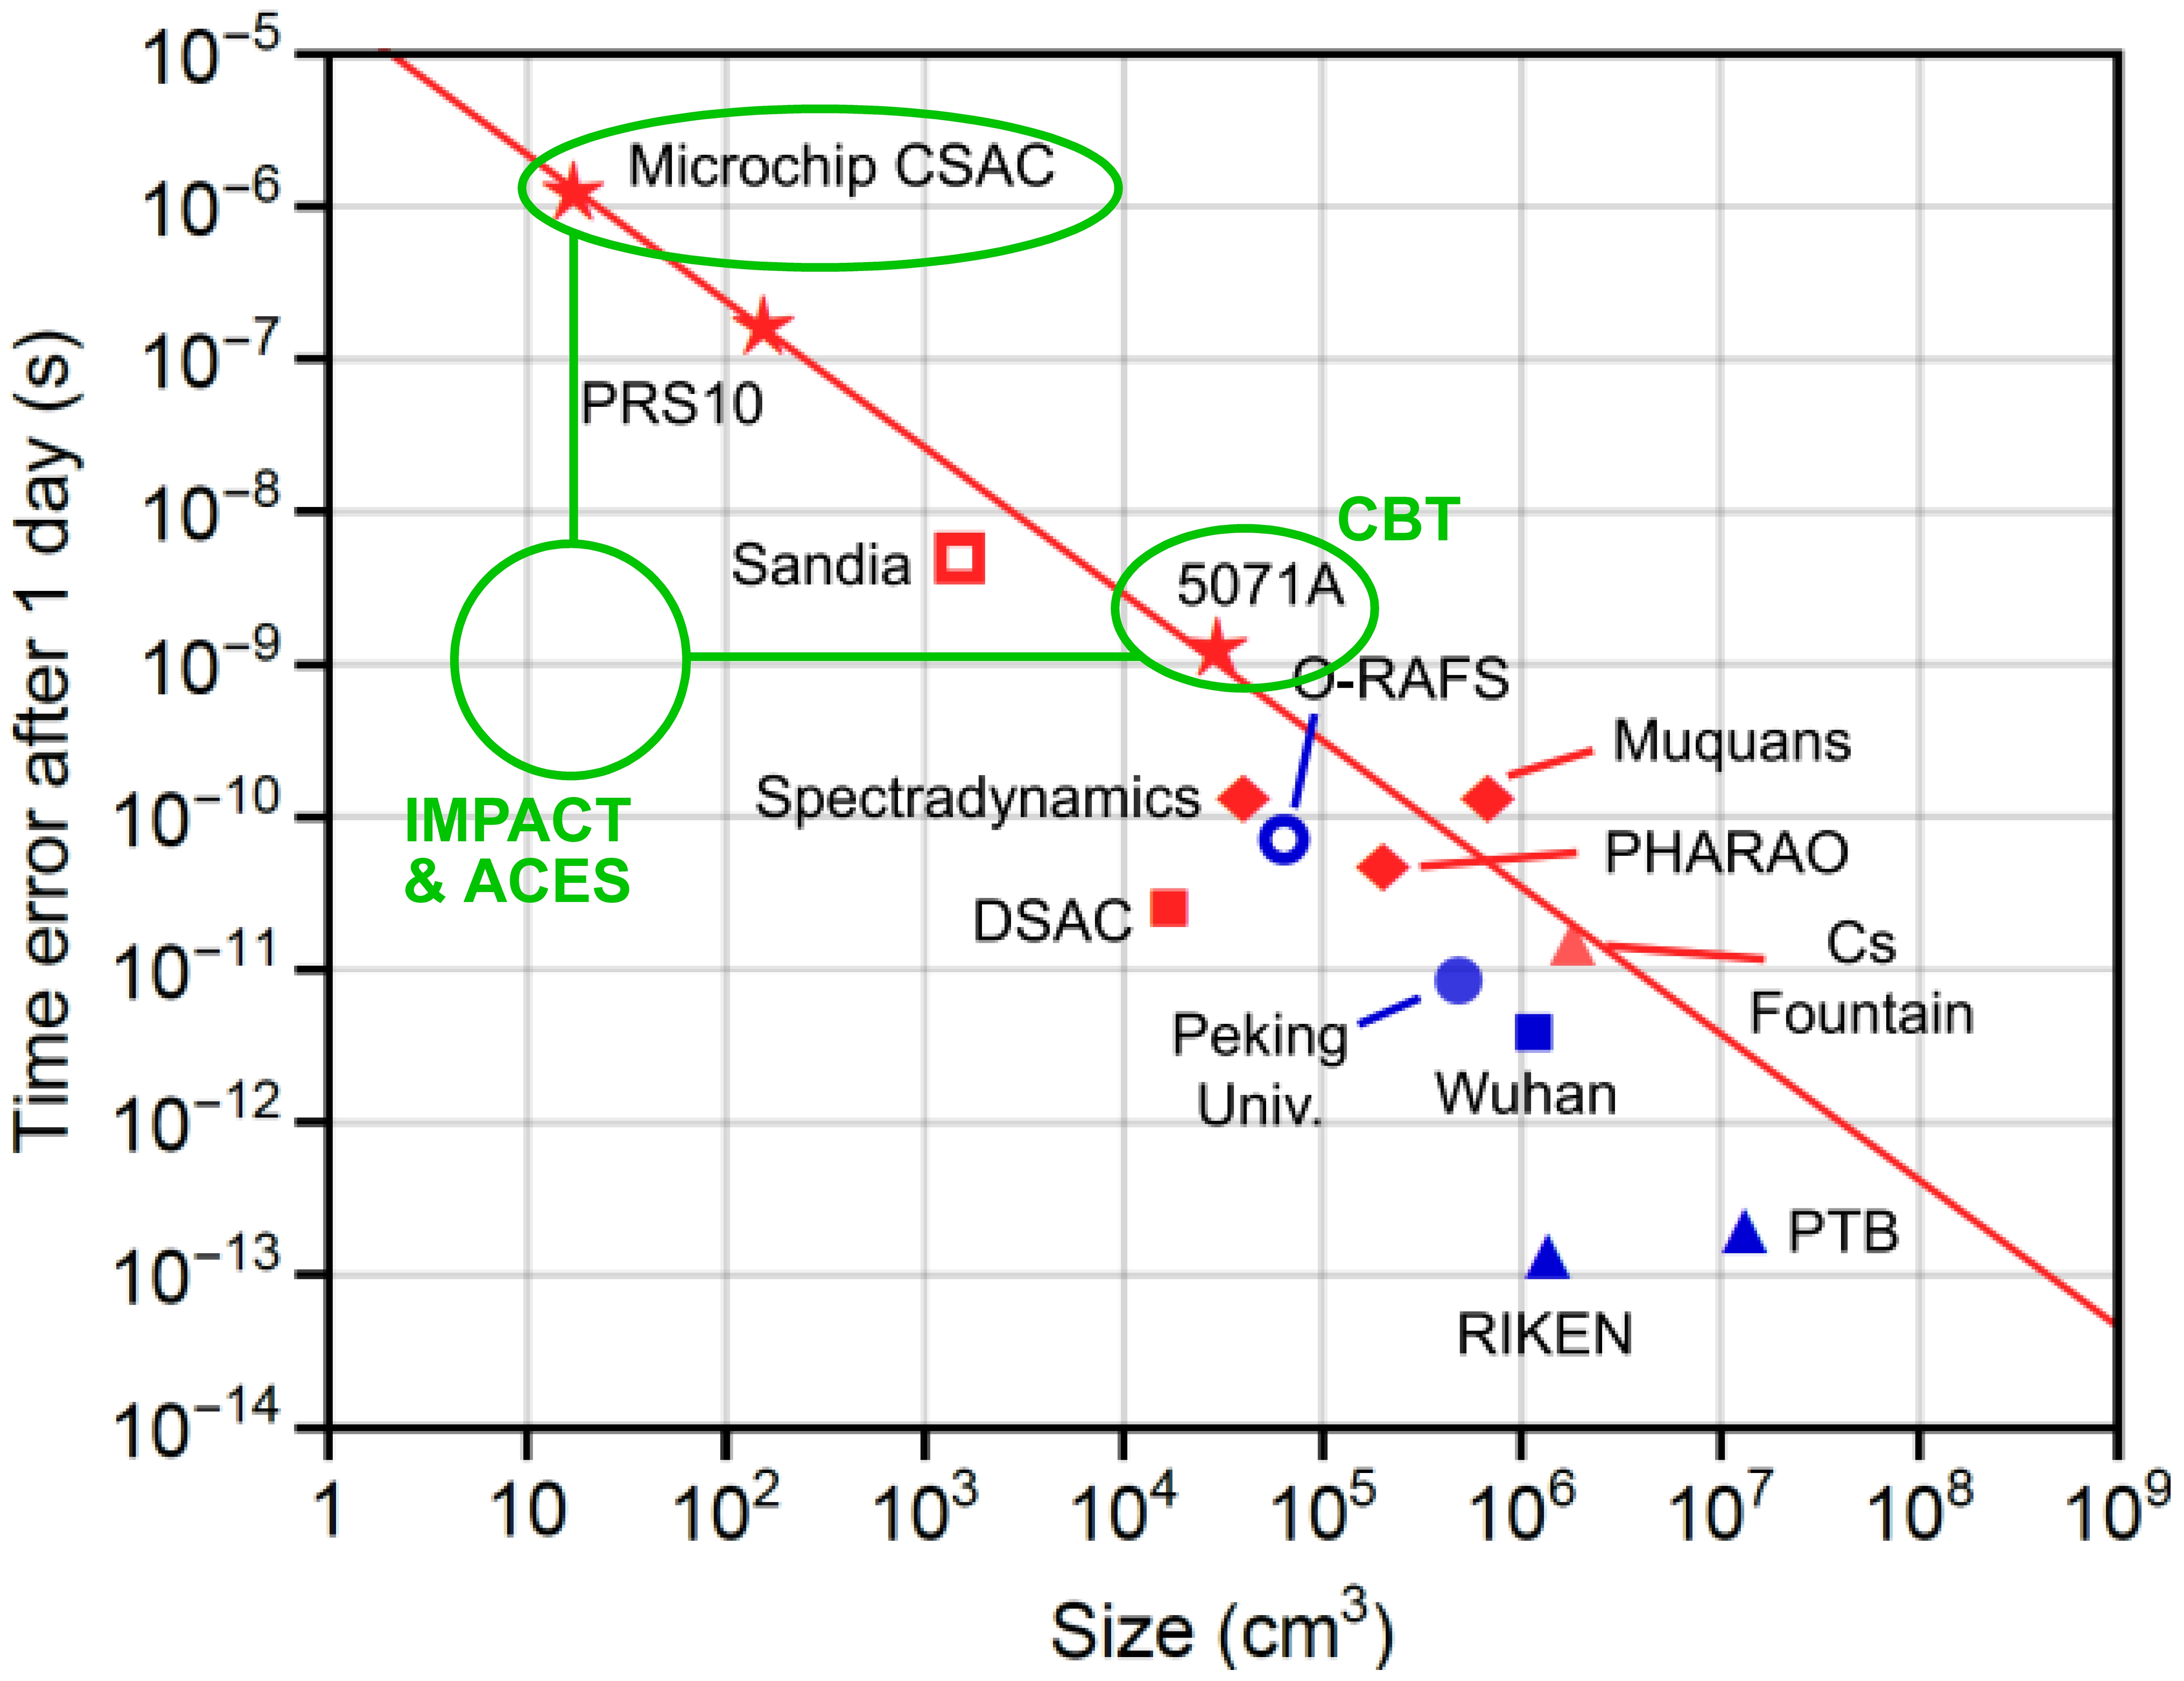
\includegraphics[width=0.6\textwidth, max width=\linewidth]{img/DARPA-stability-target.jpg}
    \caption{Stability targets for the DARPA IMPACT and ACES programs. Source \cite{Marlow-Scherer}.}
    \label{fig:DARPA-stability-target}
\end{figure}

Generally speaking, the next generation of \acrshort{csacs} aims to achieve similar quality in terms pf performances to the current Cesium Beam Tube (CBT) clocks, which are the current gold standard for high-precision timekeeping, while maintaining the advantages of the \acrshort{csac} technology in terms of size, weight and power consumption.

